\documentclass[t]{beamer}

\usepackage[english]{babel}

\usepackage{float}
%\floatstyle{boxed}
%\restylefloat{figure}
\usepackage{times}
%\usepackage[T1]{fontenc}
\usepackage{graphicx}
\usepackage{hyperref}
\usepackage{listings}
\usepackage[utf8]{inputenc}
\usepackage{graphicx}
%% \usepackage{pgf,tikz}
%% \usepackage{pgfplots}
%% \usetikzlibrary{shapes,arrows,snakes,automata,backgrounds,petri,calc,trees}
%% \usetikzlibrary{matrix, positioning, fit}
%% \usepackage{smartdiagram}
%% \usepackage{mathtools}
\usepackage{ulem}


%\setbeameroption{show only notes}

\def\PresTitle{Greybeard's Guide to *NIX}
\font\footnoteFont=phvr7t at 8pt
\font\footnoteRefFont=phvro7t at 8pt
\font\thFont=phvb7t at 12pt
\newfont{\codeFont}{cmtt10 scaled 800}
\setbeamerfont{verbatim}{size={\fontsize{8pt}{10pt}}}
\mode<presentation>
{
  \usetheme{Madrid}
  \setbeamercovered{transparent}
  \usecolortheme{orchid}
}


\title[\PresTitle]{\PresTitle}

\author[Steve Roggenkamp] % (optional, use only with lots of authors)
{Steve Roggenkamp\\
}

\date[13 Sep 2017] % (optional)
{13 Sep 2017 \\
 }

\institute[]{
 Institute for Biomedical Informatics\\
 
 University of Kentucky\\
 
 \href{mailto:steve.roggenkamp@uky.edu}{\nolinkurl{steve.roggenkamp@uky.edu}}
}

\subject{\PresTitle}

\begin{document}

\frame{\titlepage}

% \begin{frame}{}
%  \begin{itemize}
%  \item Why learn to use the command line?
%  \item Six things to know
%  \end{itemize}
% \end{frame}

\begin{frame}{Why learn to use the command line?}
  \begin{itemize}
  \item Systems administration
  \item Resource constrained systems
    \begin{itemize}
    \item Embedded systems
    \item High performance systems
    \end{itemize}
  \item It can do a lot for you
  \end{itemize}
  \note{}
\end{frame}

\begin{frame}{The Shell}
  \begin{itemize}
    \item Parses your input and executes commands
    \item Provides an environment in which you work
    \item Provides a scripting programming language
  \end{itemize}
\end{frame}

\begin{frame}{Shells - If you don't like one, try another}
  \begin{itemize}
  \item \texttt{ash}, \texttt{bash}, \texttt{dash}
  \item Bourne shell, Korn shell, PD Korn,  Bourne-again shell
  \item \texttt{csh}, \texttt{tcsh}, \texttt{zsh}
  \item Busybox (which normally uses \texttt{ash})
  \item Each provides unique set of capabilities
  \item Today's talk focuses on Bourne-again shell, aka, \texttt{bash}
    \begin{itemize}
    \item Default shell for most Linux and Mac OSX
      \item Available for most *NIX system
    \end{itemize}
  \end{itemize}
  \note{}
\end{frame}

\begin{frame}{Starting a shell}
  \begin{itemize}
  \item Log into a terminal
  \item Remotely execute a shell via \texttt{ssh}
  \item Log into a system console
  \end{itemize}
  \note{}
\end{frame}

\begin{frame}{Sample session start}
  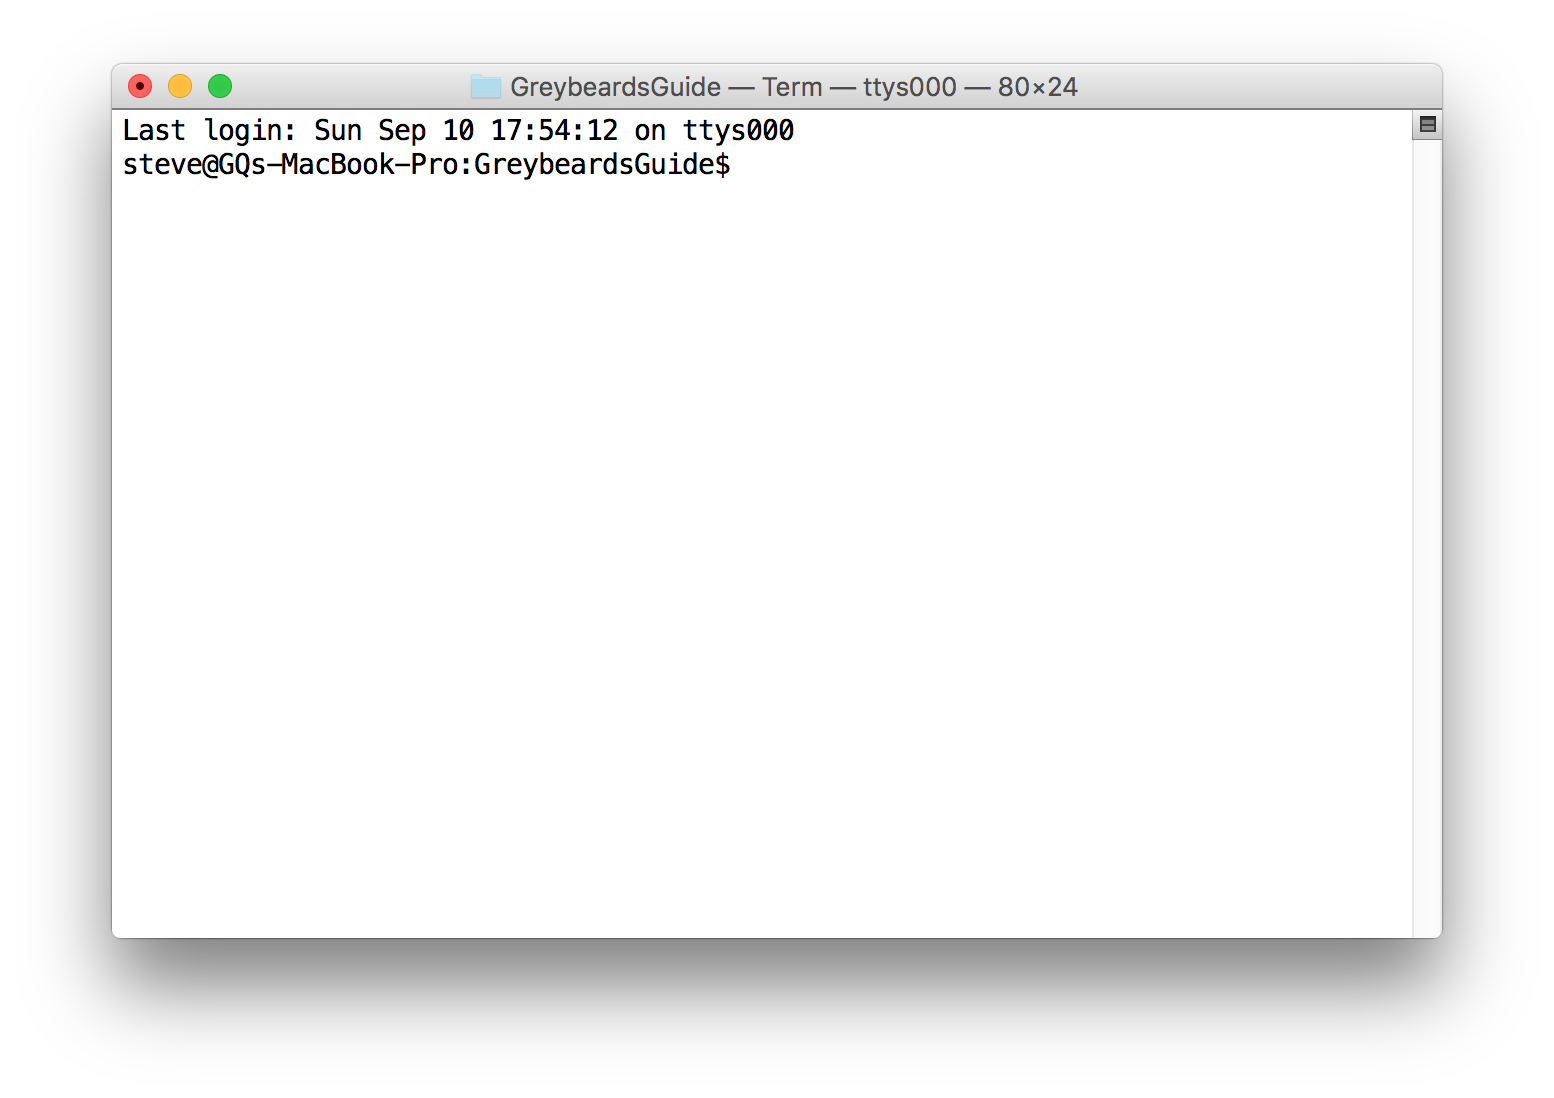
\includegraphics[width=10cm,scale=0.4]{images/newtty-1.png}

  Now what?? Coder's Block!!!
  \note{}
\end{frame}

\begin{frame}{Session - list current directory}
  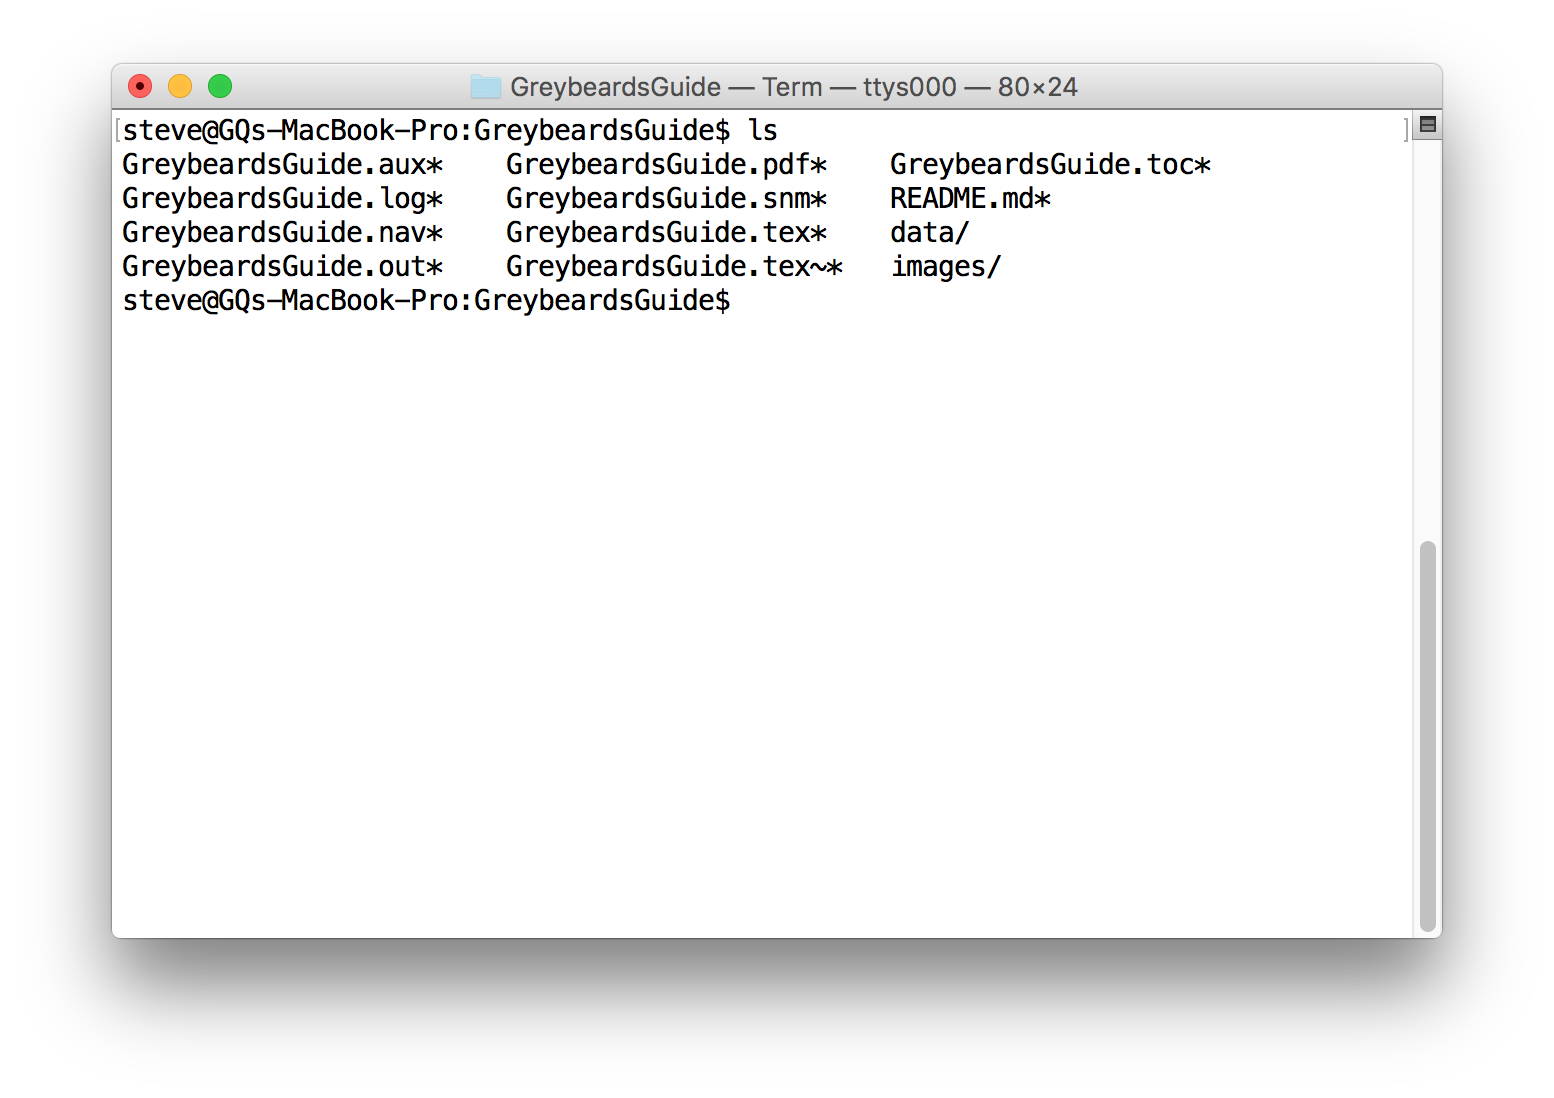
\includegraphics[width=10cm,scale=0.4]{images/newtty-2.png}

  \texttt{ls} lists the contents of a directory
  \note{}
\end{frame}


\begin{frame}{What to type for a given command}
  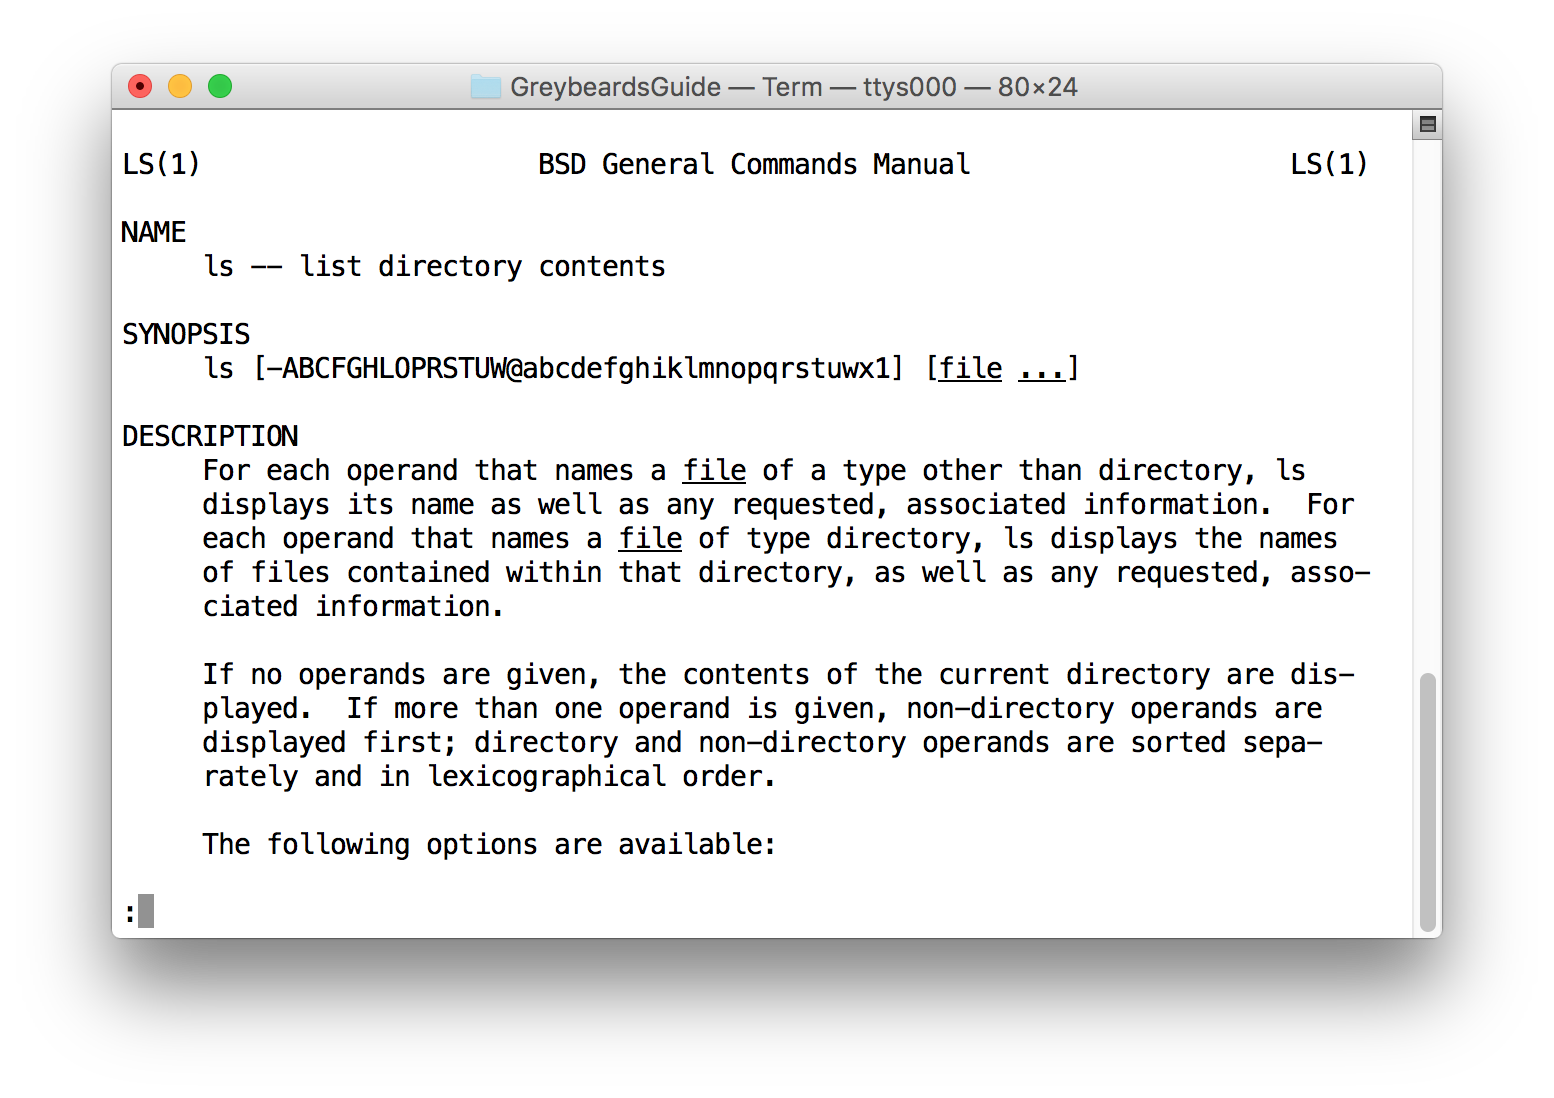
\includegraphics[width=10cm,scale=0.4]{images/newtty-3.png}

  \begin{itemize}
  \item \texttt{man ls} provides the manual page for \texttt{ls}
  \end{itemize}
  \note{}
\end{frame}

\begin{frame}{Man pages}
  \begin{itemize}
  \item \texttt{man} pages contain multiple sections
  \item Typical sections include:
    \begin{itemize}
    \item NAME - name of the command and brief discussion
    \item SYNOPSIS - how to invoke the command and list of arguments
    \item DESCRIPTION - detailed description of the program
    \item OPTIONS - options and their description
    \item EXAMPLES - example invocations and what they do
    \item EXIT STATUS - \texttt{exit(2)} codes (0 indicates success) 
    \item ENVIROMENT - how shell variables affect program
    \item SEE ALSO - other programs or documents to consult
    \item BUGS - known issues
    \end{itemize}
  \end{itemize}
  \note{}
\end{frame}

\begin{frame}{Man pages}
  \begin{itemize}
  \item UNIX documentation system
  \item Organized into multiple sections
    \begin{itemize}
    \item 1 - programs or shell commands
    \item 2 - System (kernel) calls
    \item 3 - Library calls
    \item 4 - Special files (usually found in /dev)
    \item 5 - File formats
    \item 6 - Games
    \item 7 - Miscellaneous
    \item 8 - System administration commands (root)
    \item 9 - Non-standard kernel commands
    \end{itemize}
  \end{itemize}
  \note{}
\end{frame}

\begin{frame}{Man pages - cont.}
  \begin{itemize}
  \item 
  \item 
  \item 
  \item 
  \item 
  \end{itemize}
  \note{}
\end{frame}

\begin{frame}{}
  \begin{itemize}
  \item 
  \end{itemize}
  \note{}
\end{frame}

\begin{frame}{}
  \begin{itemize}
  \item 
  \end{itemize}
  \note{}
\end{frame}

\begin{frame}{}
  \begin{itemize}
  \item 
  \end{itemize}
  \note{}
\end{frame}

\begin{frame}{}
  \begin{itemize}
  \item 
  \end{itemize}
  \note{}
\end{frame}

\begin{frame}{}
  \begin{itemize}
  \item 
  \end{itemize}
  \note{}
\end{frame}

\begin{frame}{}
  \begin{itemize}
  \item 
  \end{itemize}
  \note{}
\end{frame}

\begin{frame}{Questions?}
  \note{}
\end{frame}

\end{document}
